\section{Fundamentals of Interfacing}
\subsection{Basic Interface Structure}
\begin{minipage}{9cm}
	\begin{itemize}
		\item Power Source
		\item Clock Oscillators
		\item Power on Reset
		\item Booting Function
	\end{itemize}
\end{minipage}
\begin{minipage}{5cm}
	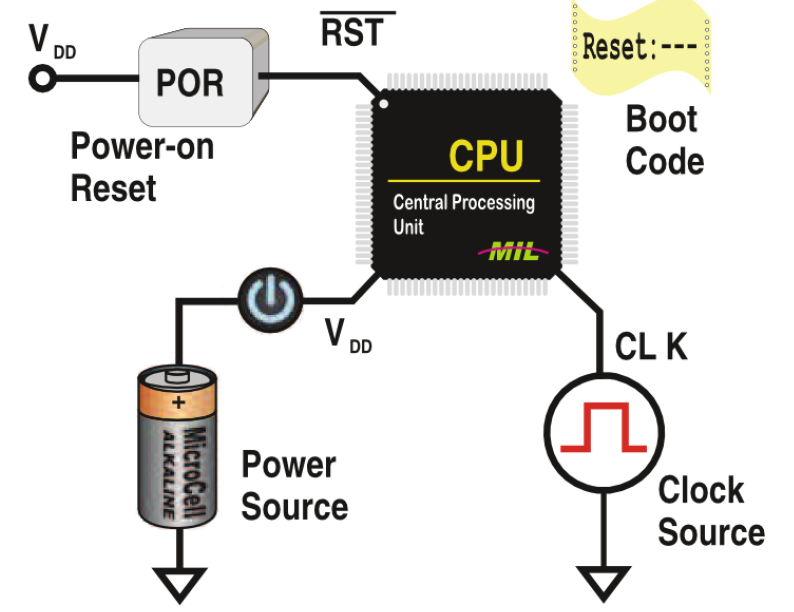
\includegraphics[width=6cm]{images/power.png}
\end{minipage}
\subsection{Power Sources}
\begin{itemize}
	\item Provide Power to CPU and Electronic
	\item Require Steady Voltage
	\item Establish reference Levels for internal Operations
	\item Absolute Maximum Ratings
	\subitem Maximum and Minimum supply values
	\subitem Level of Stress
	\subitem Do Not design operating device at these levels
	\item Recommended Operating Conditions
	\subitem Conditions where the device operating normal	
\end{itemize}
\subsection{Clock Sources}
\begin{itemize}
	\item Embedded Systems need a steady clock
	\item Synchronous nature of CPU and peripherals
	\item Time Base for bus activity, timers, baud rates etc
\end{itemize}
\subsubsection{Parameters for Clock Signal}
\begin{minipage}{9cm}
	\begin{itemize}
		\item Voltage Swing $V_{SW}=V_{OH}-V_{OL}$
		\item Frequnecy $f_{clk}=1/T_{clk}$
		\item Duty Cycle $DC=t_{high}/T_{clk} \cdot 100 \%$
		\item Edge Speed $t_r, t_f$
	\end{itemize}
\end{minipage}
\begin{minipage}{8cm}
	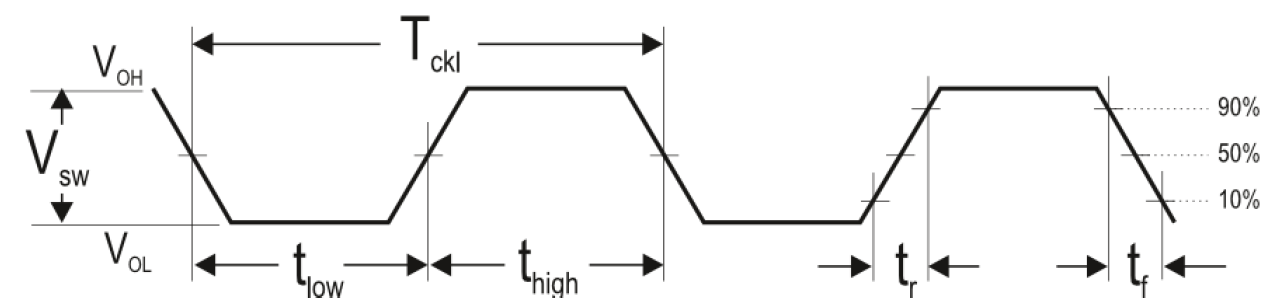
\includegraphics[width=8cm]{images/clock_parameters.png}
\end{minipage}
\clearpage
\pagebreak